%
% operation.tex
%
% Copyright (C) 2022 by SpaceLab.
%
% TTC 2.0 Critical Design Review
%
% This work is licensed under the Creative Commons Attribution-ShareAlike 4.0
% International License. To view a copy of this license,
% visit http://creativecommons.org/licenses/by-sa/4.0/.
%

%
% \brief Project management slides.
%
% \author Gabriel Mariano Marcelino <gabriel.mm8@gmail.com>
% \author Miguel Boing <miguelboing13@gmail.com>
%
% \version 0.1.0
%
% \date 2022/08/18
%


\begin{frame}{Operation}

    \begin{itemize}
        \item By default, the TTC will always operate in RX mode
        \vspace{0.3cm}
        \item If requested by an external device, a packet is transmitted (TX mode)
        \vspace{0.3cm}
        \item An external device can read or write from/to the internal parameters
        \vspace{0.3cm}
        \item The received packets are stored in a queue with five positions (up to five packets can be stored)
        \vspace{0.3cm}
        \item When requested, an external device can read the decoded packets from the queue
    \end{itemize}

\end{frame}

\begin{frame}{RF Protocol: \href{https://mgm8.github.io/pyngham/protocol.html}{\textcolor{cyan}{\underline{NGHam}}}}

    \begin{itemize}
        \item With FEC (Reed-Solomon with seven different schemes)
        \item Up to 220 bytes of data per packet
    \end{itemize}

    \begin{figure}[!ht]
        \begin{center}
            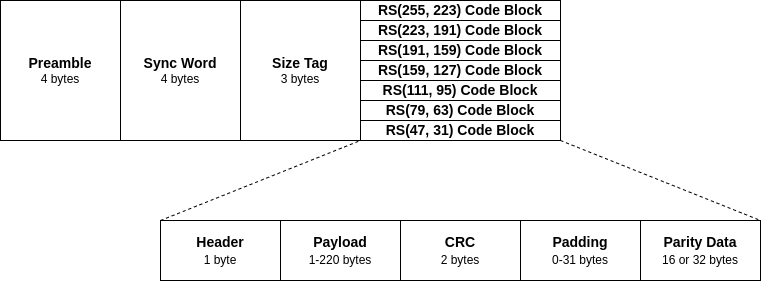
\includegraphics[width=10cm]{figures/ngham-pkt.png}
        \end{center}
    \end{figure}

\end{frame}

\begin{frame}{NGHam: Sizes}

    \begin{table}[!htb]\small
    \centering
    \label{tab:ngham-sizes}
    \begin{tabular}{cccC{1.3cm}C{1.8cm}}
        \toprule[1.5pt]
        \textbf{Size Num.} & \textbf{Tag} & \textbf{RS Config.} & \textbf{Parity Bytes} & \textbf{Max. Data Bytes} \\
        \midrule
        1 & 59, 73, 205   & RS(47, 31)   & 16 & 28 \\
        2 & 77, 218, 87   & RS(79, 63)   & 16 & 60 \\
        3 & 118, 147, 154 & RS(111, 95)  & 16 & 92 \\
        4 & 155, 180, 174 & RS(159, 127) & 32 & 124 \\
        5 & 160, 253, 99  & RS(191, 159) & 32 & 156 \\
        6 & 214, 110, 249 & RS(223, 191) & 32 & 188 \\
        7 & 237, 39, 52   & RS(255, 223) & 32 & 220 \\
        \bottomrule[1.5pt]
    \end{tabular}

\end{table}

\end{frame}

\begin{frame}{NGHam: Parameters}

    \begin{itemize}
        \item \textbf{Preamble}: 4 $\times$ 0xAA
        \item \textbf{Sync. Word}: 0x5D, 0xE6, 0x2A, 0x7E
        \item \textbf{CRC}:
        \begin{itemize}
            \item \textit{Polynomial}: 0x1021
            \item \textit{Initial value}: 0xFFFF
            \item \textit{Final XOR value}: 0xFFFF
        \end{itemize}
        \item \textbf{Reed-Solomon}:
        \begin{itemize}
            \item \textit{Symbol size}: 8
            \item \textit{GF polynomial}: 0x187 (coeficients form)
            \item \textit{First root of RS code generator polynomial}: 112 (index form)
            \item \textit{Primitive element}: 11
            \item \textit{Number of roots}: 16 or 32
        \end{itemize}
    \end{itemize}

\end{frame}

\begin{frame}{NGHam: Scrambling}
    
    \begin{itemize}
        \item Before transmitting a packet, the RS code block is scrambled by making a byte xor operation with a pre-generated table based on the polynomial $x^{8} + x^{7} + x^{5} + x^{3} + 1$ (defined in the CCSDS 131.0-B-3 standard)
        \vspace{0.5cm}
        \item When the receiver receives a packet, it also perform the same operation to de-scramble the RS code block and get the original content of the RS part of the packet
        \vspace{0.5cm}
        \item More information: \href{https://public.ccsds.org/Pubs/132x0b3.pdf}{\textcolor{blue}{\underline{CCSDS 131.0-B-3}}} (section 8.3)
    \end{itemize}

\end{frame}